\documentclass{f1rstlady/templates/presentation}
\setbeamersize{text margin left=1em,text margin right=1em}
\usepackage{csquotes}

% Source code integration
\usepackage{f1rstlady/sourcecode}
\lstset{
    language = [LaTeX]{TeX},
    inputpath = examples,
    keywordstyle = \color{Green4}}
\lstdefinestyle{custom}{
    style = context,
    basicstyle = \small\ttfamily,
    caption = {}}

% Macro to display examples
\renewcommand*{\example}[1]{
    \begin{description}
        \item[Input:]
            \lstinputlisting{#1}
        \item[Output:]
            \input{examples/#1}
    \end{description}}

% TeX workflow diagram
\usepackage{smartdiagram}

% For the biblatex example
\usepackage{xpatch} % See section "1.5.2 Recommended Packages" of the documentation
\usepackage[style=alphabetic]{biblatex}
\addbibresource{examples/bibliography.bib}
\defbibheading{bibliography}[\bibname]{} % Do not create a section at \printbibliography

% For the \DeclarePairedDelimiter example
\usepackage{mathtools}

% Information to be included in the title page:
\title{\LaTeX~Workshop}
\author{Benedikt Rips}
\institute{\LaTeX~Universität}
\date{\today}

\begin{document}

\frame[plain]{\titlepage}

\AtBeginSection[]{
    \begin{frame}
        \tableofcontents[currentsection, sectionstyle=show/shaded]
    \end{frame}}

\begin{frame}{Was ist \LaTeX?}
\begin{itemize}
    \item Ein Textsatzsystem zum Setzen ansprechender Texte mit mathematischen Inhalten.
        (Eigentlich: Erweiterung für das Textsatzsystem \TeX)
    \smallskip
    \item De\-/facto\-/Standard in Mathematik, Informatik, Naturwissenschaften und mathematiknahen
        Disziplinen
    \smallskip
    \item Kostenlose Open Source Software
\end{itemize}
\end{frame}

\begin{frame}{Warum \LaTeX?}
\LaTeX~bietet zahlreiche Vorteile gegenüber gängigen Textverarbeitungsprogrammen:
\begin{itemize}
    \item Klare Trennung von Inhalt und Formatierung
    \item Einfacheres und mächtigeres Setzen mathematischer Formeln
    \item Plattformunabhängig
    \item Flexibilität – diese Präsentation wurde mit \LaTeX~erstellt!
    \item Ausgeprägte Modularität
    \item Automatisiertes Erstellen von Abschnittsnummerierungen, Inhalts- und
        Literaturverzeichnissen, \dots
    \item Zuverlässiges Zitieren und cross referencing
    \item Programmierbar durch Kontrollstrukturen
\end{itemize}
\end{frame}

\section{Einführung}

\subsection{Ein Minimalbeispiel}

\begin{frame}{\subsecname}
\begin{itemize}
    \item Beim \enquote{\TeX{}en} verfasst man zunächst \alert{Quellcode} in einer simplen Textdatei
        mit \texttt{.tex}\-/Endung:
        \lstinputlisting[style=custom]{minimal.tex}
    \item Ein \alert{Compiler} erzeugt daraus ein gewünschtes Output\-/Format:
        \begin{center}
            \texttt{> lualatex HelloWorld.tex}
        \end{center}
    \item Es gibt verschiedene Compiler (für PDF\-/Ausgabe):
        \begin{itemize}
            \item \alert{\texttt{pdflatex}} wurde und wird immer noch viel verwendet.
            \item \alert{\texttt{lualatex}} ist moderner und gilt als dessen Nachfolger.
        \end{itemize}
        Der Compiler muss ggf. im Editor eingestellt werden.
\end{itemize}
\end{frame}

\subsection{Grober Aufbau}

\begin{frame}{\subsecname}
\begin{itemize}
    \item Eine \TeX\-/Datei (\texttt{.tex}) beginnt in der Regel mit einer sog. \alert{Präambel}:
        \lstinputlisting[style=custom]{preamble.tex}
    \item In dieser werden alle Einstellungen des Dokuments festgelegt, wie z.B. Layout, eigene
        Befehle und zusätzliche Pakete. Dies erzeugt noch keinen sichtbaren Output!
    \item Notwendig: \lstinline{\\documentclass\{...\}} zu Beginn zum Festlegen der
        \alert{Dokumentklasse}.
        \begin{itemize}
            \item Empfohlen: KOMA\-/Script\-/Klassen (\texttt{scrartcl}, \texttt{scrreprt},
                \texttt{scrbook}, \dots) statt der Standardklassen (\texttt{article},
                \texttt{report}, \texttt{book}, \dots)
        \end{itemize}
\end{itemize}
\end{frame}

\begin{frame}{Grober Aufbau (2)}
\begin{itemize}
    \item Der eigentliche Inhalt, der ausgegeben werden soll, befindet sich in der Umgebung
        \texttt{document}:
        \lstinputlisting[style=custom]{document.tex}
    \item Text nach \lstinline{\\end\{document\}} wird nicht verarbeitet.
\end{itemize}
\end{frame}

\subsection{Leerzeichen, Zeilenumbrüche \& Paragraphen}

\begin{frame}{Leerzeichen}
\begin{itemize}
    \item Wörter werden durch Leerzeichen getrennt.  Die Anzahl der Leerzeichen ist aber irrelevant:
        \example{whitespace.tex}
    \item Möchte man unbedingt ein Leerzeichen erzeugen, so muss man eine Tilde einfügen:
        \example{whitespace_non-breaking.tex}
    \item Dies ist in der Regel nicht notwendig, da \LaTeX~normalerweise automatisch den richtigen
        Abstand zwischen Wörten bestimmt.
\end{itemize}
\end{frame}

\begin{frame}{Zeilenumbrüche}
\begin{itemize}
    \item Zeilenumbrüche im Quellcode übertragen sich im Allgemeinen nicht auf die PDF:
        \example{newline.tex}
    \item Man kann durch \lstinline{\\\\} einen Zeilenumbruch erzwingen:
        \example{newline_forced.tex}
    \item Auch hier gilt: Passende Stellen für Zeilenumbrüche werden in der Regel automatisch
        bestimmt.
\end{itemize}
\end{frame}

\begin{frame}{Paragraphen}
\begin{itemize}
    \item Um Text in Paragraphen zu teilen, muss man sie im Quellcode durch eine Leerzeile trennen:
        \example{paragraph.tex}
    \item Alternativ erzeugt der Befehl \lstinline{\\par} einen neuen Paragraphen.
    \item Paragraphen werden standardmäßig nicht durch vertikalen Abstand, sondern Einrückung
        hervorgehoben.
\end{itemize}
\end{frame}

\subsection{Kommentare}

\begin{frame}{\subsecname}
\begin{itemize}
    \item Alles, was einem \enquote{\texttt{\%}} folgt, wird ignoriert und taucht nicht im
        generierten Dokument auf:
        \example{comments.tex}
    \item Dies erlaubt es, den Text mit \alert{Kommentaren} zu versehen.
    \item Nützlich, um Gedanken und Erklärungen und Notizen aufzuschreiben, die vor dem Leser
        verborgen bleiben sollen.
\end{itemize}
\end{frame}

\begin{frame}{\TeX\-/Workflow}
\begin{center}
    \smartdiagram[circular diagram:clockwise]{Quellcode schreiben, kompilieren, Output begutachten}
\end{center}
\end{frame}

\subsection{Abschnitte und Überschriften}

\begin{frame}{\subsecname}
\begin{itemize}
    \item Man kann ein Dokument in \alert{Abschnitte} unterteilen mittels
        \begin{center}
            \lstinline{\\section\{Überschrift\}}
        \end{center}
    \item Neben \lstinline{\\section} gibt es z.B. \lstinline{\\chapter}, \lstinline{\\subsection}
        und \lstinline{\\paragraph}.
    \item Die Abschnitte werden automatisch nummeriert.
    \item Zu jedem dieser Makros gibt es eine unnummmerierte Variante, die durch einen Stern
        gekennzeichnet ist:
        \begin{center}
            \lstinline{\\section*} statt \lstinline{\\section}
        \end{center}
    \item Mittels \lstinline{\\tableofcontents} erzeugt man aus den Überschriften ein
        \alert{Inhaltsverzeichnis}.
\end{itemize}
\end{frame}

\subsection{Listen, Aufzählungen, Beschreibungen}

\begin{frame}{Listen}
\begin{itemize}
    \item Ein weiteres nützliches Hilfsmittel sind \alert{Listen}. Ein hilfreiches Paket dafür ist
        \texttt{enumitem}, das wie folgt in der Präambel eingebunden werden sollte:
        \begin{center}
            \lstinline{\\usepackage[shortlabels]\{enumitem\}}
        \end{center}
    \item Eine (nicht\-/nummerierte) Liste erzeugt man mit der Umgebung \texttt{itemize}:
        \example{itemize.tex}
    \item Das Aufzählungssymbol kann lokal durch eckige Klammern (\lstinline{\\item[...]}) oder
        global in der Präambel (\lstinline{\\setlist[itemize]\{label=...\}}) gesetzt werden.
\end{itemize}
\end{frame}

\begin{frame}{Aufzählungen}
\begin{itemize}
    \item Nummerierte Listen lassen sich mit der Umgebung \texttt{enumerate} erzeugen:
        \example{enumerate.tex}
    \item Durch die eckigen Klammern nach \lstinline{\\begin\{enumerate\}} kann die Nummerierung und
        Klammerung angepasst werden.
        \begin{itemize}
            \item z.B. \lstinline{[(i)], [1)], [A.],} \dots
        \end{itemize}
\end{itemize}
\end{frame}

\begin{frame}{Beschreibungen}
\begin{itemize}
    \item Die Umgebung \texttt{description} eignet sich zur Auflistung von Begriffen mit zugehörigen
        Beschreibungen:
        \example{description.tex}
\end{itemize}
\end{frame}

\subsection{Mathematische Formeln}

\begin{frame}{\subsecname}
Mathematische Formeln können auf verschiedene Arten und Weisen im so genannten \alert{math mode}
gesetzt werden:
\begin{itemize}
    \item Innerhalb von Fließtext (\alert{inline math}) mittels \lstinline{$...$}:
        \example{inline_math.tex}
    \item Abgesetzt in einer separaten Zeile (\alert{display math}) mittels \lstinline{[...]}:
        \example{display_math.tex}
\end{itemize}
\end{frame}

\begin{frame}{Indizes und Exponenten}
\begin{itemize}
    \item Indizes:
        \example{indices.tex}
        Beachte: Für Indizes mit mehr als einem Zeichen muss der Index in geschweifte Klammern
        gesetzt werden: \lstinline{v_\{i-1\}}.
    \item Exponenten:
        \example{exponents.tex}
        Beachte: Wie bei Indizes müssen mehrere Zeichen in geschweifte Klammern gesetzt werden:
        \lstinline{n^\{k+1\}}.
\end{itemize}
\end{frame}

\begin{frame}{Mehrzeilige Formeln}
\begin{itemize}
    \item Für mehrzeilige Rechnungen bieten sich Umgebungen wie \texttt{align} an:
        \example{align.tex}
    \item Die Zeilen werden dabei anhand der \lstinline{&} ausgerichtet.
    \item Andere nützliche Umgebungen sind \texttt{equation}, \texttt{gather}, \texttt{array},
        \texttt{multiline}.
    \item Diese Umgebungen werden vom Paket \texttt{amsmath} bereitgestellt, welches daher bei
        Bedarf in der Präambel eingebunden werden muss:
        \begin{center}
            \lstinline{\\usepackage\{amsmath\}}
        \end{center}
    \item Nummerierung kann mit \lstinline{\\nonumber} pro Zeile ausgeschaltet werden – oder man
        nutzt \texttt{align*} statt \texttt{align}.
\end{itemize}
\end{frame}

\begin{frame}[t]{Mathematische Symbole}
\begin{itemize}
    \item Das Paket \texttt{amssymb} enthält weitere mathematische Symbole:
        \begin{center}
            \lstinline{\\usepackage\{amssymb\}}
        \end{center}
    \item Falls man einen Befehl für ein bestimmtes mathematisches Symbol sucht, hilft der Dienst
        \href{http://detexify.kirelabs.org/classify.html}{\alert{Detexify}} weiter:
        \begin{center}
            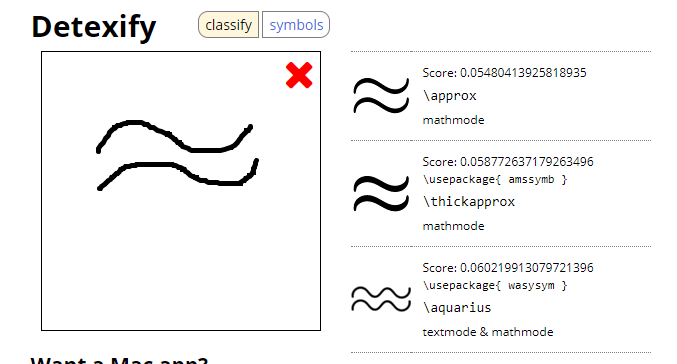
\includegraphics[keepaspectratio,width=8cm]{images/detexify.png}
        \end{center}
\end{itemize}
\end{frame}

\begin{frame}{Sätze, Lemmata und Beweise}
\begin{itemize}
    \item Um elegant und einfach Sätze, Lemmata, Beweise, etc. zu setzen, eignet sich das Paket
        \texttt{amsthm}:
        \begin{center}
            \lstinline{\\usepackage\{amsthm\}}
        \end{center}
    \item Es stellt Makros bereit um entsprechende Umgebungen zu erstellen und benutzen:
        \lstinputlisting[style=custom]{theorem.tex}
    \item Da das Erscheinungsbild in dieser Präsentation stark von dem in anderen Dokumentklassen
        abweicht, probiert es selbst mal aus.
\end{itemize}
\end{frame}

\begin{frame}{Sätze, Lemmata und Beweise (2)}
\begin{itemize}
    \item Der Befehl \lstinline{\\newtheorem\{<env_name>\}\{<name>\}} erstellt eine neue
        Theorem\-/Umgebung namens \texttt{<env\_name>}, die im Dokument als \texttt{<name>}
        erscheint.
        \begin{itemize}
            \item Damit lassen sich insbesondere Umgebungen für Lemmata, Beispiele, Bemerkungen etc.
                erstellen.
        \end{itemize}
    \item Wie für Abschnitte gibt es auch für Theorem\-/Umgebungen unnummmerierte Varianten:
        \begin{center}
            \lstinline{\\newtheorem*\{<env_name>\}\{<name>\}}
        \end{center}
        funktioniert wie \lstinline{\\newtheorem}, erstellt aber eine unnummerierte Umgebung.
\end{itemize}
\end{frame}

\section{Übung}

\subsection{Aufgabe}

\begin{frame}{\subsecname}
\begin{itemize}
    \item Im folgenden haben wir für euch ein beispielhaftes Dokument erstellt.
    \item Zu Übungszwecken empfehlen wir euch, einmal selbst zu versuchen das Dokument zu \TeX{}en.
    \medskip
    \item Bei Fragen schaut entweder auf die nächste Folie \dots
    \item \dots~oder fragt mich eben um Hilfe.
    \item Ansonsten könnt ihr auch in der Lösung nachschauen.
\end{itemize}
\end{frame}

\subsection{Wo finde ich Hilfe?}

\begin{frame}{\subsecname}
\begin{itemize}
    \item \LaTeX\ enthält bei weitem mehr Funktionalität als wir euch in diesem Workshop präsentieren
        können.
    \item Oft werdet ihr Fehler beim Kompilieren bekommen.
\end{itemize}
Deshalb ein paar Tips, wo man Hilfe und weiterführende Informationen findet:
\begin{itemize}
    \item Eine \alert{Suchmaschine} eurer Wahl mit passenden (vorzugsweise englischen) Begriffen
        oder Ausgaben des Compilers füttern.
        \begin{center}
            
\includegraphics[keepaspectratio,width=8cm]{images/google.png}
        \end{center}
    \item Auf \href{https://tex.stackexchange.com}{\alert{\TeX~StackExchange}}, einem
        Frage\-/Antwort\-/Forum
    \item In der \alert{Dokumentation} eines Pakets bzw. einer Dokumentklasse nachschauen, verfügbar
        auf \href{https://ctan.org}{CTAN}
\end{itemize}
\end{frame}

\section{Weiteres}

\subsection{Literaturverweise}

\begin{frame}{\subsecname}
\begin{itemize}
    \item Mit dem Paket \texttt{biblatex} kann man Literaturverweise einfügen.
        \lstinputlisting[style=custom]{biblatex_preamble.tex}
    \item Die Daten der referenzierten \alert{Literatur} werden in einer \texttt{.bib}\-/Datei
        angegeben:
        \lstinputlisting[style=custom]{bibliography.bib}
    \item Mit dem Befehl \lstinline{\\cite[<suffix>]\{<id>\}} erstellt man einen \alert{Verweis} auf
        den Eintrag mit der angegebenen ID, das Suffix wird angehängt:
        \example{biblatex.tex}
    \item Die Zitierweise kann man anpassen (s. Dokumentation von \texttt{biblatex}).
\end{itemize}
\end{frame}

\subsection{Referenzen}

\begin{frame}{\subsecname}
\begin{itemize}
    \item Wie vorher gesehen, werden z.B. Formeln mit der Umgebung \texttt{equation} nummeriert.  Im
        restlichen Dokument kann man nun darauf \alert{referenzieren}:
        \example{references.tex}
    \item Mit \lstinline{\\label\{<name>\}} definiert man an der Stelle der Nummerierung ein
        \alert{Label}, auf das man später mit \lstinline{\\ref\{<name>\}}  verweisen kann.
        \begin{itemize}
            \item Spezialfall: \lstinline{\\eqref\{<name>\}} bei Gleichungen und Formeln
        \end{itemize}
    \item Dies funktioniert mit allem, was nummeriert wird, z.\,B. Abschnitten und Figuren.
\end{itemize}
\end{frame}

\subsection{Eigene Makros}

\begin{frame}{\subsecname}
\begin{itemize}
    \item Wenn man denselben Text/dieselbe Konstruktion häufig nutzt, kann es manchmal nützlich
        sein, dafür ein neues \alert{Makro} zu erstellen:
        \example{macro_iprod.tex}
    \item Der Befehl \lstinline{\\newcommand\{\\macro\}[n]\{...\#1...\#2...\#n...\}}
        \begin{itemize}
            \item erstellt ein Makro namens \lstinline{\\macro}
            \item mit $n$ Argumenten,
            \item auf die im sog. \textit{Body} mit \lstinline{\#1}, \lstinline{\#2}, \dots,
                \lstinline{\#n} referenziert wird.
        \end{itemize}
        Es wird aufgerufen durch \lstinline{\\macro\{arg1\}\{arg2\}...\{argn\}}
    \item Im obigen Beispiel wird \lstinline{\\iprod\{v\}\{w\}} ersetzt durch
        \begin{center}
            \lstinline{\\left\\langle v, w \\right\\langle}
        \end{center}
\end{itemize}
\end{frame}

\begin{frame}{Eigene Makros (für mathematische Formeln)}
\begin{itemize}
    \item Mit dem Paket \texttt{mathtools} kann man kinderleicht eigene Makros für Klammern und
        Operatoren definieren.
    \item Klammern: \lstinline{\\DeclarePairedDelimiter\{\\macro\}\{<left>\}\{<right\}}.
        \example{macro_iprod_paired-delimiter.tex}
        \begin{itemize}
            \item Vorteil: Es ist einfach, die Größe der Klammern zu ändern (s. Dokumentation von
                \texttt{mathtools}).
        \end{itemize}
    \item Operatoren: \lstinline{\\DeclareMathOperator\{\\macro\}\{<name>\}}.
        \lstinputlisting[style=custom]{macro_operator.tex}
        \begin{itemize}
            \item Vorteil: Der Abstand zwischen dem Operator und dem Operanden ist korrekt.
        \end{itemize}
\end{itemize}
\end{frame}

% TODO: Einbindung von Source Code mit lstlistings
%\subsection{Source Code}

\end{document}
